%%
%% prog-folien
%%
%% Slides for my Java programming tutorial using LaTeX beamer.
%%
%% Copyright (c) 2015-2016 YouniS Bensalah <younis.bensalah@riseup.net>
%%
%% This work is released to the public domain.
%% For the full copyright and license information, please view the LICENSE file.
%%

%% LaTeX-Beamer template for KIT design
%% by Erik Burger, Christian Hammer
%% title picture by Klaus Krogmann
%%
%% version 2.1
%%
%% mostly compatible to KIT corporate design v2.0
%% http://intranet.kit.edu/gestaltungsrichtlinien.php
%%
%% Problems, bugs and comments to
%% burger@kit.edu

\documentclass[18pt]{beamer}

%% SLIDE FORMAT

% use 'beamerthemekit' for standard 4:3 ratio
% for widescreen slides (16:9), use 'beamerthemekitwide'

\usepackage{templates/beamerthemekit}
% \usepackage{templates/beamerthemekitwide}

\usepackage[utf8]{inputenc}
\usepackage{hyperref}
\usepackage{listings}
\usepackage{color}
%\usepackage{xcolor}
%\usepackage{colortbl}
%\usepackage{array}
%\usepackage{tikz}
%\usetikzlibrary{calc,shapes.multipart,chains,arrows}

%\definecolor{lime}{HTML}{8FFF53}

\newcommand{\quotes}[1]{``#1''}

%% TITLE PICTURE

% if a custom picture is to be used on the title page, copy it into the 'logos'
% directory, in the line below, replace 'mypicture' with the
% filename (without extension) and uncomment the following line
% (picture proportions: 63 : 20 for standard, 169 : 40 for wide
% *.eps format if you use latex+dvips+ps2pdf,
% *.jpg/*.png/*.pdf if you use pdflatex)

\titleimage{greendrop}

%% TITLE LOGO

% for a custom logo on the front page, copy your file into the 'logos'
% directory, insert the filename in the line below and uncomment it

%\titlelogo{mylogo}

% (*.eps format if you use latex+dvips+ps2pdf,
% *.jpg/*.png/*.pdf if you use pdflatex)

%% TikZ INTEGRATION

% use these packages for PCM symbols and UML classes
% \usepackage{templates/tikzkit}
% \usepackage{templates/tikzuml}

% the presentation starts here

\title[Exceptions]{Programmieren:\\ Exceptions}
\subtitle{Tutorium 30}
\author{YouniS Bensalah}
\date{December 18, 2015}

\institute{Chair for Software Design and Quality}

% Bibliography

\usepackage[citestyle=authoryear,bibstyle=numeric,hyperref,backend=biber]{biblatex}
\addbibresource{templates/example.bib}
\bibhang1em

\begin{document}

% change the following line to "ngerman" for German style date and logos
\selectlanguage{english}

%title page
\begin{frame}
\titlepage
\end{frame}

%table of contents
\begin{frame}{Heute}
\tableofcontents
\end{frame}

\section{Organisatorisches}

\begin{frame}{Termine}
    \textbf{Vorlesung}
    \begin{itemize}
        \item Die Vorlesung am 23.12.2015 entfällt.
        \item Die erste Vorlesung 2016 findet am 13.01.2016 statt.
    \end{itemize}

    \textbf{Tutorien}
    \begin{itemize}
        \item Die Tutorien finden im Jahr 2015 bis zum 22.12.2015 statt.
        \item Die Tutorien im Jahr 2016 beginnen ab dem 13.01.2016.
    \end{itemize}
\end{frame}

\section{Exceptions}



\begin{frame}{Exceptions}
    \begin{block}{}
        \begin{itemize}
            \item \textit{Exceptions} dienen der Ankündigung und Behandlung von \textbf{Ausnahmesituationen} (e.g., Fehler, unerwartete Ergebnisse) innerhalb eines Programms.
            \item Dabei kann die Information über die Ausnahmesituation an eine andere Programmebene zur Behandlung übergeben werden.
        \end{itemize}
    \end{block}

\end{frame}

\begin{frame}{Exceptions}
    \textit{Was passiert jetzt also bei einem Fehler ?}
    \vspace{.2in}
    \begin{enumerate}
        \item Das Programm meldet den Vorfall in dem es eine \textbf{Exception} \textit{wirft}.
        \item Der \quotes{normale} Kontrollfluss wird unterbrochen und es wird nach einem Zuständigen gesucht, der den Fehler behandelt.
        \item Wenn dieser existiert, dann wird die Exception \textit{aufgefangen} und der entsprechende Code wird ausgeführt (z. B. der Fehler wird geloggt, das Programm wird terminiert\dots).
    \end{enumerate}
\end{frame}


\subsection{try und catch}


\begin{frame}[fragile]{try-catch}
    \begin{itemize}
        \item In den \textbf{try}-Block kommt der Code, der potentiell eine Exception wirft.
        \item Im \textbf{catch}-Block steht dann der Code, der die Exception behandelt, falls eine auftritt.
        \item Nach dem \textbf{try-catch}-Block steht der Code, welcher anschließend \\
        \textit{in jedem Fall} ausgeführt wird.
    \end{itemize}

    \begin{exampleblock}{Syntax}
        \begin{lstlisting}[language=Java,basicstyle=\scriptsize]
try {
    ... // code that might throw an exception
} catch (ExceptionType e) {
    ... // code that handles the exception
}
... // code that will be executed after try-catch block
        \end{lstlisting}

    \end{exampleblock}
\end{frame}

\subsection{Exception werfen mit throw}


\begin{frame}[fragile]{throw}
    \textit{Wann wird eine Exception geworfen ?}
    \begin{itemize}
        \item Java wirft einige Exceptions automatisch, wenn etwas zur Laufzeit schiefläuft\dots
        \begin{itemize}
            \item \texttt{Integer.parseInt()} wirft eine \texttt{NumberFormatException}, falls das Argument keine gültige Zahl darstellt.
        \end{itemize}
        \item Man kann auch selbst Exceptions werfen ! (mit \texttt{throw})
    \end{itemize}

    \begin{exampleblock}{Syntax}
throw new SomeExceptionType();
    \end{exampleblock}

    \begin{itemize}
        \item Es wird also ein \textbf{Objekt} vom Typ \texttt{SomeExceptionType} erstellt und geworfen !
    \end{itemize}

\end{frame}


\begin{frame}[fragile]{Exceptions}
    Was wird hier ausgegeben ?
    \begin{exampleblock}{}
        \begin{lstlisting}[language=Java,basicstyle=\scriptsize]
public static void main(String[] args) {
    try {
        doSomething();
    } catch (ArrayIndexOutOfBoundsException e) {
        System.out.println("Oh noes!");
    }
    System.out.println("Whatever.");
}

public static void doSomething() {
    int[] foo = new int[4];
    foo[4] = 1337;
    System.out.println("I know arrays.");
}
        \end{lstlisting}

    \end{exampleblock}

\end{frame}

\begin{frame}[fragile]{Exceptions}
    \begin{block}{Output}
        \begin{lstlisting}
Oh noes!
Whatever.
        \end{lstlisting}

    \end{block}

    \pause

    \begin{itemize}
        \item Die Zeile \begin{lstlisting}[language=Java,basicstyle=\scriptsize]
foo[4] = 1337;
        \end{lstlisting}
        löst eine \texttt{ArrayIndexOutOfBoundsException} aus.
        \item Der Kontrollfluss springt in den \texttt{catch}-Block, der diese Ausnahme abfängt.
        \item Anschließend geht es \textbf{\alert{nach dem \texttt{catch}}} weiter !
        \item Die Ausgabe \quotes{\texttt{I know arrays.}} wird somit nie erreicht.

    \end{itemize}

\end{frame}


\begin{frame}[fragile]{Exceptions}
    Was wird hier ausgegeben ?
    \begin{exampleblock}{}
        \begin{lstlisting}[language=Java,basicstyle=\scriptsize]
public static void main(String[] args) {
    try {
        doMagic(42);
        System.out.println("Okay, I fixed it!");
    } catch (MagicException e) {
        System.out.println("Wrong magic.");
    }
    System.out.println("Whatever.");
}

public static void doMagic(int magic) {
    if (magic != 1337) {
        throw new MagicException();
    }
    System.out.println("Do magic...");
}
        \end{lstlisting}

    \end{exampleblock}

\end{frame}

\begin{frame}[fragile]{Exceptions}
    \begin{block}{Output}
        \begin{lstlisting}[language=Java]
Wrong magic.
Whatever.
        \end{lstlisting}

    \end{block}

\end{frame}

\begin{frame}{Exceptions}
    \alert{\huge{\textsc{Nach einer aufgefangenen Exception geht es immer nach catch weiter !!!}}}
\end{frame}

\subsection{Checked versus Unchecked}


\begin{frame}{Eigene Exceptions}
    \begin{itemize}
        \item Man kann die \quotes{built-in} Exceptions von Java verwenden:
        \begin{itemize}
            \item \texttt{IllegalArgumentException}
            \item \texttt{UnsupportedOperationException}
            \item \texttt{IndexOutOfBoundsException}
            \item \texttt{IllegalStateException}
            \item \dots
        \end{itemize}
        \vspace{.2in}
        \item Benötigt man eigene Exceptions, kann man die Klasse \texttt{Exception} bzw. \texttt{RuntimeException} \textbf{erweitern}.
    \end{itemize}

\end{frame}


\begin{frame}{Checked vs. Unchecked Exceptions}
    In Java gibt es \textbf{checked} und \textbf{unchecked} Exceptions.
    \vspace{.2in}
    \begin{itemize}
        \item \textbf{Checked Exceptions}
        \begin{itemize}
            \item Ausnahmesituation oder Problem, dessen Ursache \textbf{außerhalb} des Zuständigkeitsbereichs des aktuellen Moduls liegt
            \item \textit{Ungültige Benutzereingabe, Datenbank-Problem, keine Netzwerkverbindung, nicht vorhandene Datei \dots}
            \item Müssen \textbf{immer} abgefangen werden und durch \texttt{throws} kenntlich gemacht werden
            \item Unterklassen von \texttt{Exception}
        \end{itemize}
    \end{itemize}

\end{frame}

\begin{frame}{Checked vs. Unchecked Exceptions}

    \begin{itemize}
        \item \textbf{Unchecked Exceptions}
        \begin{itemize}
            \item Ausnahmesituation oder ungültiger Zustand, dessen Ursache meistens ein Bug im Programmcode selbst ist
            \item In den meisten Fällen kann das Programm dann ohnehin nicht sinnvoll weiterlaufen
            \item \textit{Ungültige Argumente, division by 0, ungültiger Index bei Zugriff auf Array \dots}
            \item Können, müssen aber nicht abgefangen werden
            \item Unterklassen von \texttt{RuntimeException}
        \end{itemize}
    \end{itemize}

\end{frame}


\begin{frame}{Checked vs. Unchecked Exceptions}

    \begin{itemize}
        \item \texttt{RuntimeException} ist auch Unterklasse von \texttt{Exception}.
    \end{itemize}


    \vspace{.2in}

    \begin{figure}
        
\includegraphics[scale=.5]{img/whoa.jpg}
    \end{figure}

\end{frame}

\begin{frame}[fragile]{throws}

    \begin{itemize}
        \item Methoden, die \textbf{checked Exceptions} werfen können, müssen mit \texttt{throws} kenntlich gemacht werden.
    \end{itemize}


    \begin{exampleblock}{Syntax}
        \begin{lstlisting}[language=Java,basicstyle=\scriptsize]
public void foo() throws SomeCheckedException {
    ...
}
        \end{lstlisting}

    \end{exampleblock}

\end{frame}

\begin{frame}{Exceptions}
    \begin{itemize}
        \item Eine \textbf{Exception} ist eine \alert{Ausnahmesituation !}
        \item \textbf{Exceptions} sollten nicht den normalen Kontrollfluss steuern
    \end{itemize}
\end{frame}

\begin{frame}{Javadoc @throws}
    Alle Exceptions sollten mittels \texttt{@throws} im Javadoc-Kommentar kurz erklärt werden:
    \begin{itemize}
        \item Was bedeutet diese Exception für das Programm
        \item Wann wird sie von der Methode \quotes{geworfen}
    \end{itemize}
\end{frame}


\begin{frame}{Fragen ?}
    \begin{figure}
        
\includegraphics[scale=.5]{img/question_to_idea.jpg}
    \end{figure}
\end{frame}

\section{Programmieraufgabe}

\begin{frame}{Programmieraufgabe}
    \Large{Enough theory (;}
\end{frame}

\begin{frame}{Collatz}
    Das war ja zu einfach\dots
\end{frame}

\begin{frame}{Super List 9K}
    \textbf{Super List 9K} soll eine verbesserte Version der bereits bekannten \textit{verketteten Liste} werden.

    \begin{itemize}
        \item Diesmal \textbf{doppelt} verkettete Liste
        \item Natürlich mit \textbf{Generics !}
    \end{itemize}

\end{frame}

\begin{frame}{Super List 9K}
    \dots \textit{und so sieht die Schnittstelle aus:}
    \vspace{.2in}
    \begin{itemize}
        \item \texttt{addFirst()} und \texttt{addLast()} fügen ein Element an den Anfang bzw. das Ende der Liste ein.
        \item \texttt{remove()} löscht alle Elemente aus der Liste, die mit der \texttt{equals()}-Methode gleich einem gegebenen Element sind.
        \item \texttt{contains()} prüft nach, ob ein Element in der Liste vorhanden ist.
        \item \texttt{size()} gibt die Länge der Liste (Anzahl Elemente) aus.
        \item \texttt{count()} zählt, wie oft ein Element in der Liste vorkommt.
    \end{itemize}
\end{frame}


\begin{frame}[fragile]{Super List 9K}
    \begin{enumerate}
        \item Download and unzip the template\\ \url{http://younishd.fr/prog/superlist9k-template.zip}
        \item Think\dots
        \item Write code
        \item Compile and test:\\
        \begin{lstlisting}[language=Java,basicstyle=\scriptsize]
% javac superlist9k/SuperCell.java \\
        superlist9k/SuperList.java \\
        superlist9k/SuperListInterface.java \\
        test/SuperTest.java

% java test.SuperTest
        \end{lstlisting}
        \item Repeat \texttt{2-4} until all tests are \textcolor{green}{green}!
    \end{enumerate}
\end{frame}

\begin{frame}{Super List 9K}
    Die Lösung findet Ihr hier:
    \begin{itemize}
        \item \url{http://younishd.fr/prog/superlist9k.zip}
    \end{itemize}
\end{frame}

\appendix
\beginbackup

\begin{frame}{Bis nächstes Jahr !}
    \begin{figure}
        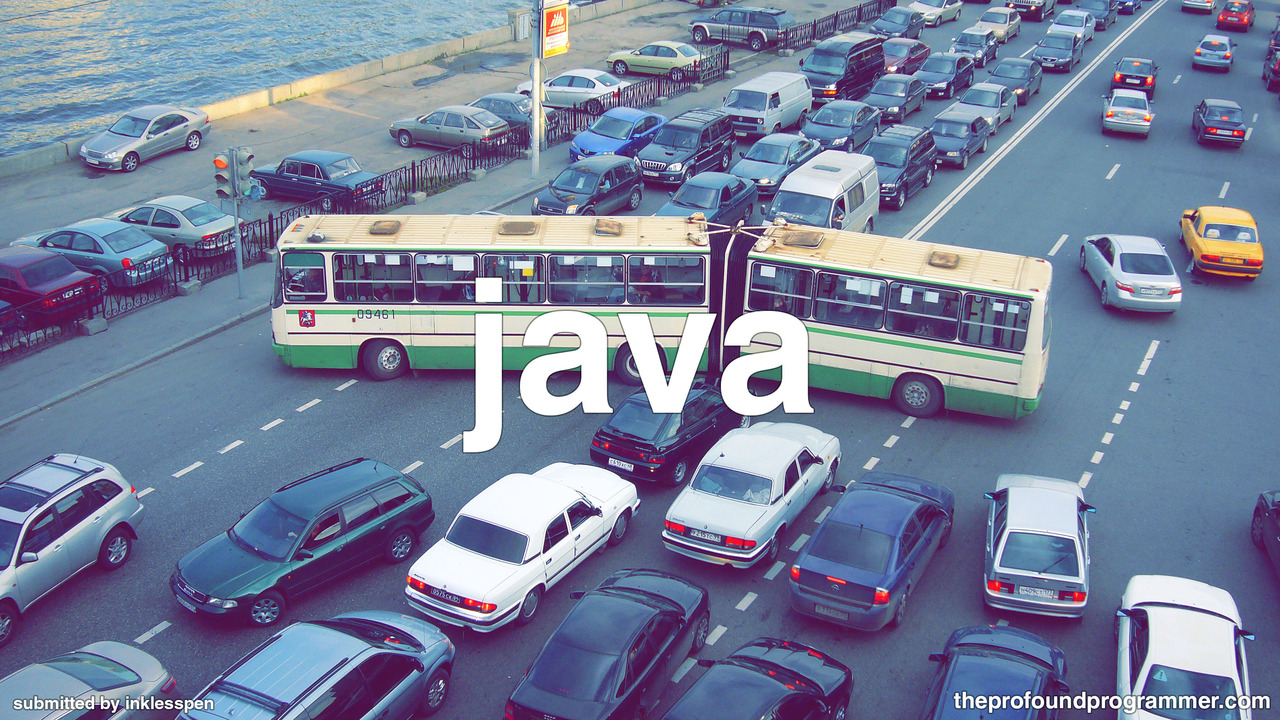
\includegraphics[scale=.25]{img/java.jpg}
    \end{figure}
\end{frame}

\backupend

\end{document}
